\documentclass[a4paper,11pt,fleqn]{article}%fleqn pour aligner les equations à gauche
\usepackage{/home/rweye/Nextcloud/Documents/Overleaf/Styles/Cours}

\newcommand{\chnum}{Chapitre 2}
\newcommand{\chtitle}{Concentration en masse de sucre dans une boisson commerciale}
\newcommand{\dtype}{TP}
	
  
\begin{document}
\maketitle
\textbf{Objectif : Le sucre est très présent dans un grand nombre de boissons. Comment vérifier la concentration massique en sucre d’une boisson ?}\\
\begin{figure}[h!]
\fbox{
\begin{minipage}{.7\textwidth}
	\caption{Une canette d'une boisson bien connue et sa composition}
	\begin{center}
		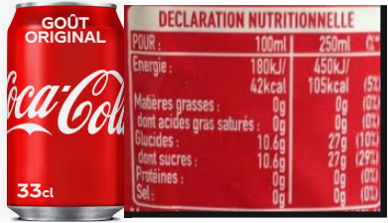
\includegraphics[scale=.5]{Ressources/2GT_C4_AE2_Fig1.png}
	\end{center}
\end{minipage}
\begin{minipage}{.3\textwidth}
	\caption{Matériel disponible}
	\begin{itemize*}
		\item Balance
		\item Fiole jaugée de 50 mL
		\item Éprouvette graduée de 50 mL
		\item Béchers
		\item Bouteille de boisson
		\item Pipette plastique
	\end{itemize*}
\end{minipage}}

\fbox{
\begin{minipage}{.5\textwidth}
	\caption{Qu'est ce qu'une courbe d'étalonnage ?}
	Une courbe d’étalonnage permet de faire le lien entre deux grandeurs physiques. La série de mesures nécessaires pour l’établir permet d’avoir une meilleure précision sur le résultat final que si l’on réalise une mesure unique.\\
\textit{Exemple : courbe $P=f(m)$ montrant le lien graphique entre le poids $P$ d’un objet et sa masse $m$.}
\end{minipage}
\begin{minipage}{.5\textwidth}
	\begin{center}
		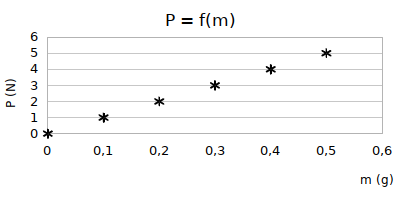
\includegraphics[scale=.6]{Ressources/2GT_C4_AE2_Fig2.png}
	\end{center}
\end{minipage}
}
\end{figure}

\section*{Travail à réaliser}
\begin{enumerate}
	\item Quelle différence y a t il entre la masse volumique et la concentration massique ?
	\item Pourquoi, selon vous, arrive-t-il que la masse volumique et la concentration en masse d’une solution soient confondues ?
	\item Pour mieux comprendre le lien qu’il y a entre ces deux grandeurs, on souhaite étudier comment évolue la masse volumique d’une solution aqueuse de saccharose en fonction de la concentration en masse de saccharose.
	\begin{enumerate}
		\item Quelle formule permet de calculer la masse de soluté à utiliser pour préparer une solution, si on connaît le volume à préparer et la concentration en masse de soluté ?
		\item Compléter la quatrième ligne du tableau suivant :
	\end{enumerate}
		\begin{tabular}{|>{\centering}m{2cm}|>{\centering}m{1.5cm}|>{\centering}m{1.5cm}|>{\centering}m{1.5cm}|>{\centering}m{1.5cm}|>{\centering}m{1.5cm}|>{\centering}m{1.5cm}|>{\centering}m{1.5cm}|>{\centering\arraybackslash}m{1.5cm}|}
		\hline N° solution & 1 & 2 & 3 & 4 & 5 & 6 & 7 & 8\\
		\hline $V_{solution}$ (\unit{\milli \liter}) & 50& 50& 50& 50& 50& 50& 50& 50\\
		\hline $\gamma_{saccharose}$ (\unit{\gram \per \liter}) & 10 & 20 & 40 & 60 & 80 & 100 & 120 & 140\\
		\hline $m_{saccharose}$ (\unit{\gram})& & & & & & & & \\
		\hline $\rho_{solution}$ (\unit{\gram \per \liter})& & & & & & & & \rule[.8cm]{0cm}{0cm}\\
		\hline \end{tabular}
	\begin{enumerate}
\setcounter{enumii}{2}
			\item Proposer un protocole expérimental permettant de déterminer la masse volumique de l’une de ses solutions.
			\item Réaliser le protocole et compléter le tableau précédent.
			\item À l'aide des résultats obtenus, tracer la représentation graphique de $\rho = f(\gamma_{saccharose})$ sur un tableur informatique.
	\end{enumerate}
	\item Proposer un protocole permettant de déterminer la valeur de concentration de la boisson sucrée, sans utiliser les informations données par l'étiquette.
	\item Après accord du professeur, mettre en \oe uvre  le protocole proposé. Indiquer précisément les mesures et calculs réalisés.
	\item À l'aide du \textbf{Document 1}, calculer la concentration en masse de sucre théorique de la boisson proposée. L'exprimer en \unit{\gram \per \liter}.
	\item Comparer la valeur expérimentale à la valeur théorique et calculer le pourcentage d'écart entre les deux valeurs en utilisant la formule suivante :
	$$\text{écart en \% = } \dfrac{valeur_{\text{théorique}}-valeur_{\text{expérimentale}}}{valeur_{\text{théorique}}} \times 100$$
\end{enumerate}
\end{document}